\section{Background}
\label{sec:background}

\begin{figure*}
    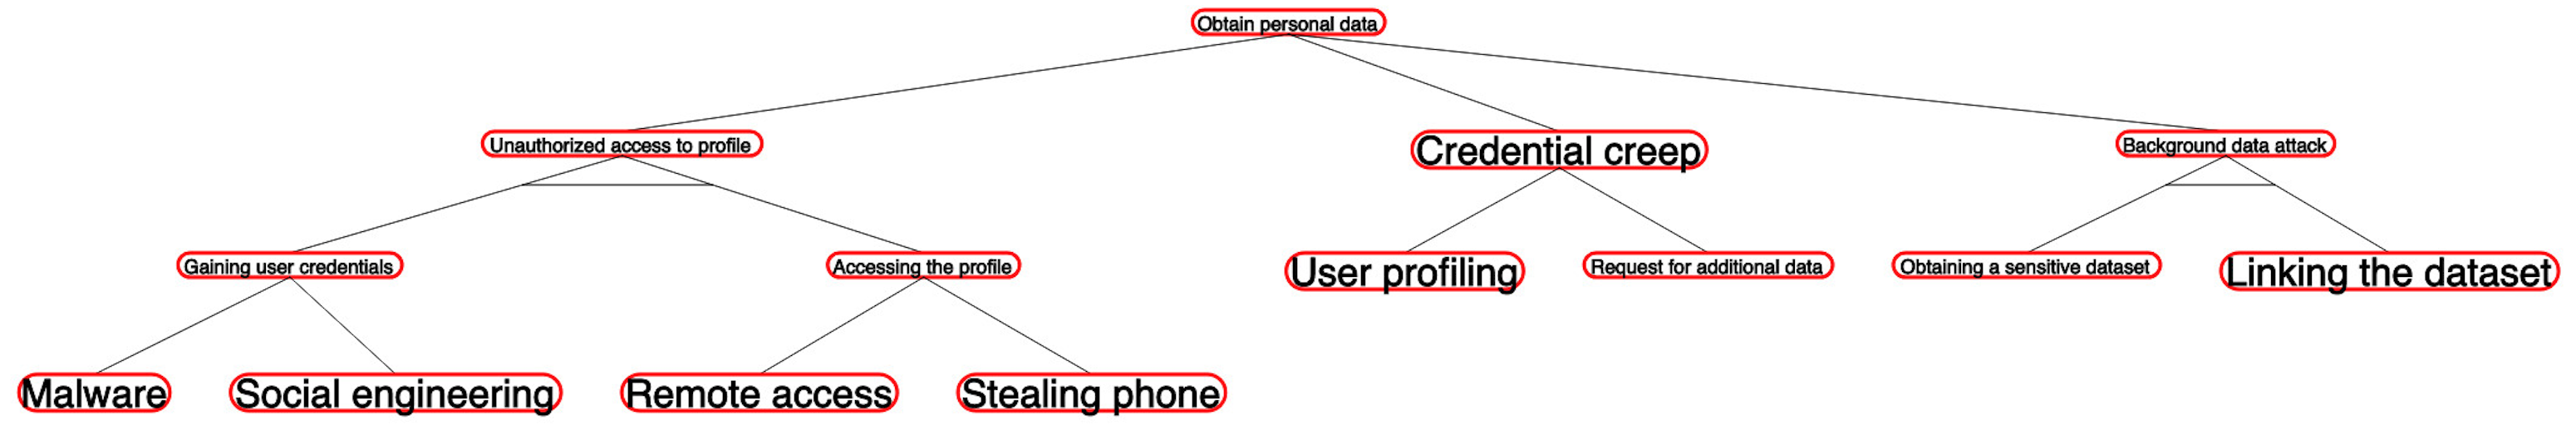
\includegraphics[width=\linewidth]{img/TargetAT.png}
    \caption{An attack tree adapted from Naik \etal~\cite{naikEvaluationPotentialAttack2022} that is used in the study described in Section~\ref{sec:methodology}. }
    \label{fig:tartgetAT}
\end{figure*}

We define attack trees to be a rooted acyclic structure with the following recursive definition adapted from Gadyatskaya~\etal~\cite{gadyatskayaRefinementAwareGenerationAttack2017}.

\begin{definition} \label{def:attack-tree} An attack tree  is defined as $T = \ATnode{1}{1}\Delta(\ATnode{2}{1},...,\ATnode{2}{i})$. Where $\ATnode{d}{i} = \ATlabel{d}{i}\Delta(\ATnode{d+1}{j},...,\ATnode{d+1}{k})$

    % We define the $i\text{th}$ node according to left-right post-order number to be the following, $T[i] = b\Delta(T[j],...,T[k])$. 

    % We give $b$ to be some action within the attack scenario, which is the node label of $t$. For clarity, we additionally refer to this label as $t.\text{label}$. We give $\Delta$ to be the refinement $\Delta = \AND|\OR|\SAND$. For clarity and consistency, we refer to the refinement of a given node to be $t.\Delta$. Following the refinement, we have a list of nodes which are the children of $t$, defined as $t_0,...,t_i$ which is the left to right order of the children (regardless of if order is significant). We refer to the list of children as $t.\text{children}$. This list of nodes can be empty, in the case of leaf nodes.

    % For clarity and consistency, we refer to the refinement of a given node to be $t.\Delta$. Following the refinement, we have a list of nodes which are the children of $\ATnode{d}{i}$, defined as $\ATnode{d+1}{j},...,\ATnode{d+1}{k}$ where $j \ge 1$ and $k \ge j$, which is the left to right order of the children (regardless of if order is significant). We refer to the list of children as $\ATnode{d}{i}.\text{children}$. This list of nodes can be empty, in the case of leaf nodes.

    Each node within an attack tree is a sub-tree unto itself. We define each node as $\ATnode{d}{i}$ where $d$ is the depth of the node (distance from the root, given the root has a starting distance of 1), and $i$ is the number of that node counting from the left most node at depth $d$ (starting from 1). We define a mapping of each node to a label space, where the label of node $\ATnode{d}{i}$ is given as $\ATlabel{d}{i}$. We give $\Delta$ to be the refinement $\Delta = \AND|\OR$. We further define the following functions to retrieve associated information of some node $\ATnode{d+1}{j}$. We define the $\Delta(\ATnode{d}{i})$ function to return the refinement of a given node. We define the child function, $\childFunc{\ATnode{d}{i}}$ to return a list of nodes which are the children of a given node, defined as $\ATnode{d+1}{j},...,\ATnode{d+1}{k}$ where $j \ge 1$ and $k \ge j$, which is the left to right order of the children (regardless of if order is significant). This list of nodes can be empty, in the case of leaf nodes. Finally, we define the parent function, $\parentFunc{\ATnode{d}{i}}$ to return the parent of a given node.
\end{definition}
